% ------------------------------------------------------------------------
% file `main-bookexercise-2-exercise-body.tex'
%
%     exercise of type `bookexercise' with id `2'
%
% generated by the `exercise' environment of the
%   `xsim' package v0.21 (2022/02/12)
% from source `main' on 2026/10/10 on line 1137
% ------------------------------------------------------------------------
    1. [多选]下列说法正确的是$\underline{\hspace{1cm}}$。\\
A. 栈是一种有特殊要求的线性表。\\
B. 队列是一种有特殊要求的线性表。\\
C. 最先入栈的元素一定最先出栈。\\
D. 最先入队的元素一定最先出队。\\

    2. 以下哪一项不是栈可以进行的操作？$\underline{\hspace{1cm}}$\\
A. 将元素压入栈中\\
B. 判断栈是否为空\\
C. 删除栈底元素\\
D. 将栈置为空栈\\

    3. 以下哪一项不是队列可以进行的操作？$\underline{\hspace{1cm}}$\\
A. 将元素插入队尾\\
B. 获取队首元素的值\\
C. 获取位序为i的元素的值\\
D. 位序为i的元素出队\\

    4. 某个栈，元素的入栈序列是 $$ 1,2,3,4 $$ 则以下序列中，不可能作为出栈序列的是：$\underline{\hspace{1cm}}$\\
A. 2, 1, 3, 4\\
B. 2, 3, 4, 1\\
C. 3, 2, 4, 1\\
D. 3, 4, 1, 2\\

    5. 关于时间复杂度，以下说法正确的是：\\
A. 顺序栈的 Push 和 Pop 时间均为 \(O(n)\)\\
B. 链栈的 Push 和 Pop 均可实现为 \(O(1)\)\\
C. 使用单链表实现队列时，只要有 head 指针，入队和出队均可实现为 \(O(1)\)\\
D. 循环队列的入队操作必须移动大量元素，因此时间复杂度为 O(n)\\

    6. 采用数组实现容量为 \(N\) 的循环队列，并规定：\\
front 指向队首元素；\\
rear 指向下一个插入位置；\\
front和rear初始全部指向下标\(N-1\)处，队列采用保留一个空闲位置的方式区分队满和队空。

则判断队列为空和队满的条件分别为：\\
A. front == 0 \&\& rear == 0, rear + 1 == front\\
B. front == 0 \&\& rear == 0, (rear + 1) \% N == front\\
C. front == rear, rear + 1 == front\\
D. front == rear, (rear + 1) \% N == front \\

    7. [多选]某同学做了如下设计：采用一个长度为100的数组实现两个栈S1和S2。该同学规定两栈栈底分别在两个端点处，栈顶向中间生长，如图\ref{fig:共享栈}。
    同时规定两栈栈顶元素相邻时，存储空间满，均无法再入栈。
\begin{figure}[htbp]
    \centering
    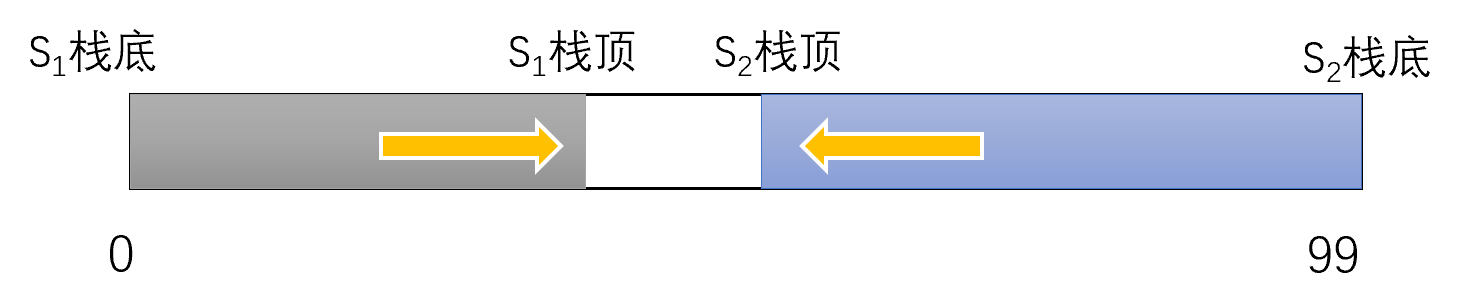
\includegraphics[width=0.67\textwidth]{assets/pics_and_ppts/ch3/共享栈.png}
    \caption{}
    \label{fig:共享栈}
\end{figure}
    以下说法中正确的是$\underline{\hspace{1cm}}$\\\\
\textbf{A.} 两栈入栈时间复杂度均为O(1)\\
\textbf{B.} 设两栈元素数量分别为n、m，则两栈栈顶元素的出栈时间复杂度分别为O(n)、O(m)\\
\textbf{C.} 要计算两栈栈中已有元素数量之和，时间复杂度为O(1)\\\\
\textbf{D.} 若S1.top初始化为-1，S2.top初始化为100，且两个栈顶指针始终指向各自的栈顶元素，则S1.top+1==S2.top时，空间满，两栈均无法再入栈\\
\textbf{E.} 若S1.top初始化为-1，S2.top初始化为100，且两个栈顶指针始终指向各自的栈顶元素，则可能出现S1.top>S2.top\\
\textbf{F.} 若S1.top初始化为0，S2.top初始化为99，且两个栈顶指针始终指向各自栈顶元素的下一个位置，则S1.top+1==S2.top时，空间满，两栈均无法再入栈\\
\textbf{G.} 若S1.top初始化为0，S2.top初始化为99，且两个栈顶指针始终指向各自栈顶元素的下一个位置，则可能出现S1.top>S2.top\\


    8. 一个初始为空的栈和一个初始为空的队列，都依次接收：
$$ 1,2,3,4,5 $$
如果只允许进行正常的入栈、出栈、入队、出队操作，关于它们能够产生的输出顺序，下列说法正确的是：\\
A. 栈和队列都可以产生任意排列\\
B. 栈只能产生一种输出顺序，队列也只能产生一种输出顺序\\
C. 队列的输出顺序固定为 \(1,2,3,4,5\)，而栈的输出顺序受到栈操作过程限制\\
D. 栈的输出顺序固定为 \(5,4,3,2,1\)，队列的输出顺序受到操作过程限制\\

    9.[多选]假设输入序列是1,2,3,4,5，利用两个队列进行出入队操作，不可能的输出序列有$\underline{\hspace{1cm}}$\\
A. 5,4,3,2,1\\
B. 5,1,2,3,4\\
C. 5,2,3,1,4\\
D. 2,3,4,5,1\\

    10. [多选]与循环队列相比，链式队列$\underline{\hspace{1cm}}$\\
A. 优点是进队和出队时间复杂度更低\\
B. 优点是长度可以在内存限制内动态变化\\
C. 缺点是节点除数据外需要额外的存储空间存放指针\\
D. 缺点是不能根据队首和队尾指针以O(1)时间算出队列长度\\

    11. 假设某队列采用带头结点的循环双链表实现，第一个数据节点表示队头，最后一个数据节点表示队尾。若只设头指针指向头节点，则进队和出队的时间复杂度分别为：\\
A. O(1), O(1) \\
B. O(1), O(n)\\
C. O(n), O(1)\\
D. O(n), O(n)\\

    12. （某年408真题）现有队列Q和栈S，初始时Q中的元素依次是1,2,3,4,5,6（1在队头），S为空。若仅允许下列的3种操作：\Circled{1}出队并输出出队元素；\Circled{2}出队
    并将出队元素入栈；\Circled{3}出栈并输出出栈元素。则不能得到的输出序列是$\underline{\hspace{1cm}}$\\
A. 1,2,5,6,4,3\\
B. 2,3,4,5,6,1\\
C. 3,4,5,6,1,2\\
D. 6,5,4,3,2,1\\

    13. （某年408真题）某队列允许在其两端进行入队操作，但仅允许在一端进行出队操作。若元素a,b,c,d,e依次入此队列后再进行出队操作，则不可能得到的出队序列是$\underline{\hspace{1cm}}$\\
A. b,a,c,d,e\\
B. d,b,a,c,e\\
C. d,b,c,a,e\\
D. e,c,b,a,d\\

    14. （某年408真题）初始为空的队列Q的一端仅能进行入队操作，另外一端既能进行入队操作，又能进行出队操作。若Q的入队序列是1,2,3,4,5，则不能得到的出队序列是$\underline{\hspace{1cm}}$\\
A. 5,4,3,1,2\\
B. 5,3,1,2,4\\
C. 4,2,1,3,5\\
D. 4,1,3,2,5\\

    15. （某年408真题）假设栈初始为空，将中缀表达式a/b+(c*d-e*f)/g转换为等价的后缀表达式的过程中，当扫描到f时，栈中的元素依次是$\underline{\hspace{1cm}}$\\
A. +(*-\\
B. +(-*\\
C. /+(*-*\\
D. /+-*\\

    16. （某年408真题）若栈S1中保存整数，栈S2中保存运算符，函数F()依次执行下述的各步操作：\\
    1) 从S1中依次弹出两个操作数a和b；\\
    2) 从S2中弹出一个运算符op；\\
    3) 执行相应的运算b op a；\\
    4) 将运算结果压入S1中。\\
    假定S1中的操作数依次是5,8,3,2（2在栈顶），S2中的运算符依次是*, -, +（+在栈顶）。调用3次F()后，S1栈顶保存的值是$\underline{\hspace{1cm}}$\\
    A. -15\\
    B. 15\\
    C. -20\\
    D. 20\\

    *17. 某游戏服务器持续记录某位名为CoreLoop的玩家的网络延迟情况。现假设服务器连续记录了 \(n\) 个时刻的网络延迟，第 \(i\) 个时刻的延迟为 delay[i]，
    这些数值均为正整数。为防止数值闪动，该服务器将时刻i的近k个时刻延迟的最大值作为该玩家在时刻i的\textbf{显示延迟}。
    也就是说，时刻i的显示延迟为：
    \[
        max(delay[max(0, i-k+1)], delay[max(0, i-k+2)], ..., delay[i])
    \]

    如，对于：
    \[
        delay[] = {40, 33, 38, 37, 42, 35}
    \]

    k=3时，显示延迟为
    \[
        ans[]   = {40, 40, 40, 38, 42, 42}
    \]

    k=4时，显示延迟为
    \[
        ans[]   = {40, 40, 40, 40, 42, 42}
    \]
    请你设计一个尽可能高效的算法，求出该玩家这n个时刻的\textbf{显示延迟}。
    \begin{cppcode}
    // 将时刻0到n-1的显示延迟保存在ans[]数组下标0到n-1处。
        void MaxDelay(int delay[], int n, int k, int ans[]) {

        }
    \end{cppcode}



